\documentclass{article}
\usepackage[left=1in,right=1in]{geometry}
\usepackage{subfiles}
\usepackage{amsmath, amssymb, stmaryrd, verbatim} % math symbols
\usepackage{amsthm} % thm environment
\usepackage{mdframed} % Customizable Boxes
\usepackage{hyperref,nameref,cleveref,enumitem} % for references, hyperlinks
\usepackage[dvipsnames]{xcolor} % Fancy Colours
\usepackage{mathrsfs} % Fancy font
\usepackage{bbm} % mathbb numerals
\usepackage{tikz, tikz-cd, float} % Commutative Diagrams
\usetikzlibrary{decorations.pathmorphing} % for squiggly arrows in tikzcd
\usepackage{perpage}
\usepackage{parskip} % So that paragraphs look nice
\usepackage{ifthen,xargs} % For defining better commands
\usepackage[T1]{fontenc}
\usepackage[utf8]{inputenc}
\usepackage{tgpagella}
\usepackage{cancel}

% Bibliography
\usepackage{url}
\usepackage{biblatex}

\addbibresource{mybib.bib}

% Shortcuts

% % Local to this project
\renewcommand\labelitemi{--} % Makes itemize use dashes instead of bullets

% % Misc
\newcommand{\brkt}[1]{\left(#1\right)}
\newcommand{\sqbrkt}[1]{\left[#1\right]}
\newcommand{\dash}{\text{-}}

% % Logic
\renewcommand{\implies}{\Rightarrow}
\renewcommand{\iff}{\Leftrightarrow}
\newcommand{\limplies}{\Leftarrow}
\newcommand{\NOT}{\neg\,}
\newcommand{\AND}{\, \land \,}
\newcommand{\OR}{\, \lor \,}
\newenvironment{forward}{($\implies$)}{}
\newenvironment{backward}{($\limplies$)}{}

% % Sets
\DeclareMathOperator{\supp}{supp}
\newcommand{\set}[1]{\left\{#1\right\}}
\newcommand{\st}{\,|\,}
\newcommand{\minus}{\setminus}
\newcommand{\subs}{\subseteq}
\newcommand{\ssubs}{\subsetneq}
\newcommand{\sups}{\supseteq}
\newcommand{\ssups}{\supset}
\DeclareMathOperator{\im}{Im}
\newcommand{\nothing}{\varnothing}
\DeclareMathOperator{\join}{\sqcup}
\DeclareMathOperator{\meet}{\sqcap}

% % Greek 
\newcommand{\al}{\alpha}
\newcommand{\be}{\beta}
\newcommand{\ga}{\gamma}
\newcommand{\de}{\delta}
\newcommand{\ep}{\varepsilon}
\newcommand{\ph}{\varphi}
\newcommand{\io}{\iota}
\newcommand{\ka}{\kappa}
\newcommand{\la}{\lambda}
\newcommand{\om}{\omega}
\newcommand{\si}{\sigma}

\newcommand{\Ga}{\Gamma}
\newcommand{\De}{\Delta}
\newcommand{\Th}{\Theta}
\newcommand{\La}{\Lambda}
\newcommand{\Si}{\Sigma}
\newcommand{\Om}{\Omega}

% % Mathbb
\newcommand{\A}{\mathbb{A}}
\newcommand{\C}{\mathbb{C}}
\newcommand{\F}{\mathbb{F}}
\newcommand{\G}{\mathbb{G}}
\newcommand{\M}{\mathbb{M}}
\newcommand{\N}{\mathbb{N}}
\renewcommand{\P}{\mathbb{P}}
\newcommand{\Q}{\mathbb{Q}}
\newcommand{\R}{\mathbb{R}}
\newcommand{\U}{\mathbb{U}}
\newcommand{\V}{\mathbb{V}}
\newcommand{\Z}{\mathbb{Z}}

% % Mathcal
\newcommand{\BB}{\mathcal{B}}
\newcommand{\CC}{\mathcal{C}}
\newcommand{\DD}{\mathcal{D}}
\newcommand{\EE}{\mathcal{E}}
\newcommand{\FF}{\mathcal{F}}
\newcommand{\GG}{\mathcal{G}}
\newcommand{\HH}{\mathcal{H}}
\newcommand{\II}{\mathcal{I}}
\newcommand{\JJ}{\mathcal{J}}
\newcommand{\KK}{\mathcal{K}}
\newcommand{\LL}{\mathcal{L}}
\newcommand{\MM}{\mathcal{M}}
\newcommand{\NN}{\mathcal{N}}
\newcommand{\OO}{\mathcal{O}}
\newcommand{\PP}{\mathcal{P}}
\newcommand{\QQ}{\mathcal{Q}}
\newcommand{\RR}{\mathcal{R}}
\newcommand{\TT}{\mathcal{T}}
\newcommand{\UU}{\mathcal{U}}
\newcommand{\VV}{\mathcal{V}}
\newcommand{\WW}{\mathcal{W}}
\newcommand{\XX}{\mathcal{X}}
\newcommand{\YY}{\mathcal{Y}}
\newcommand{\ZZ}{\mathcal{Z}}

% % Mathfrak
\newcommand{\f}[1]{\mathfrak{#1}}

% % Mathrsfs
\newcommand{\s}[1]{\mathscr{#1}}

% % Category Theory
\DeclareMathOperator{\obj}{Obj}
\DeclareMathOperator{\END}{End}
\DeclareMathOperator{\AUT}{Aut}
\newcommand{\CAT}{\mathbf{Cat}}
\newcommand{\SET}{\mathbf{Set}}
\newcommand{\TOP}{\mathbf{Top}}
\newcommand{\MON}{\mathbf{Mon}}
\newcommand{\GRP}{\mathbf{Grp}}
\newcommand{\AB}{\mathbf{Ab}}
\newcommand{\RING}{\mathbf{Ring}}
\newcommand{\CRING}{\mathbf{CRing}}
\newcommand{\MOD}{\mathbf{Mod}}
\newcommand{\VEC}{\mathbf{Vec}}
\newcommand{\ALG}{\mathbf{Alg}}
\newcommand{\PSH}{\mathbf{PSh}}
\newcommand{\SH}{\mathbf{Sh}}
\newcommand{\ORD}{\mathbf{Ord}}
\newcommand{\POSET}{\mathbf{PoSet}}
\newcommand{\id}[1]{\mathbbm{1}_{#1}}
\newcommand{\map}[2]{\yrightarrow[#2][2.5pt]{#1}[-1pt]}
\newcommand{\iso}[1][]{\cong_{#1}}
\newcommand{\op}{^{op}}
\newcommand{\darrow}{\downarrow}
\newcommand{\LIM}{\varprojlim}
\newcommand{\COLIM}{\varinjlim}
\DeclareMathOperator{\coker}{coker}
\newcommand{\fall}[2]{\downarrow_{#2}^{#1}}
\newcommand{\lift}[2]{\uparrow_{#1}^{#2}}

% % Algebra
\newcommand{\nsub}{\trianglelefteq}
\newcommand{\inv}{^{-1}}
\newcommand{\dvd}{\,|\,}
\DeclareMathOperator{\ev}{ev}

% % Analysis
\newcommand{\abs}[1]{\left\vert #1 \right\vert}
\newcommand{\norm}[1]{\left\Vert #1 \right\Vert}
\renewcommand{\bar}[1]{\overline{#1}}
\newcommand{\<}{\langle}
\renewcommand{\>}{\rangle}
\renewcommand{\hat}[1]{\widehat{#1}}
\renewcommand{\check}[1]{\widecheck{#1}}
\newcommand{\dsum}[2]{\sum_{#1}^{#2}}
\newcommand{\dprod}[2]{\prod_{#1}^{#2}}
\newcommand{\del}[2]{\frac{\partial#1}{\partial#2}}
\newcommand{\res}[2]{{% we make the whole thing an ordinary symbol
  \left.\kern-\nulldelimiterspace % automatically resize the bar with \right
  #1 % the function
  %\vphantom{\big|} % pretend it's a little taller at normal size
  \right|_{#2} % this is the delimiter
  }}

% % Galois
\DeclareMathOperator{\gal}{Gal}
\DeclareMathOperator{\Orb}{Orb}
\DeclareMathOperator{\Stab}{Stab}
\newcommand{\emb}[3]{\mathrm{Emb}_{#1}(#2, #3)}
\newcommand{\Char}[1]{\mathrm{Char}#1}

%% code from mathabx.sty and mathabx.dcl to get some symbols from mathabx
\DeclareFontFamily{U}{mathx}{\hyphenchar\font45}
\DeclareFontShape{U}{mathx}{m}{n}{
      <5> <6> <7> <8> <9> <10>
      <10.95> <12> <14.4> <17.28> <20.74> <24.88>
      mathx10
      }{}
\DeclareSymbolFont{mathx}{U}{mathx}{m}{n}
\DeclareFontSubstitution{U}{mathx}{m}{n}
\DeclareMathAccent{\widecheck}{0}{mathx}{"71}

% Arrows with text above and below with adjustable displacement
% (Stolen from Stackexchange)
\newcommandx{\yaHelper}[2][1=\empty]{
\ifthenelse{\equal{#1}{\empty}}
  % no offset
  { \ensuremath{ \scriptstyle{ #2 } } } 
  % with offset
  { \raisebox{ #1 }[0pt][0pt]{ \ensuremath{ \scriptstyle{ #2 } } } }  
}

\newcommandx{\yrightarrow}[4][1=\empty, 2=\empty, 4=\empty, usedefault=@]{
  \ifthenelse{\equal{#2}{\empty}}
  % there's no text below
  { \xrightarrow{ \protect{ \yaHelper[ #4 ]{ #3 } } } } 
  % there's text below
  {
    \xrightarrow[ \protect{ \yaHelper[ #2 ]{ #1 } } ]
    { \protect{ \yaHelper[ #4 ]{ #3 } } } 
  } 
}

% xcolor
\definecolor{darkgrey}{gray}{0.10}
\definecolor{lightgrey}{gray}{0.30}
\definecolor{slightgrey}{gray}{0.80}
\definecolor{softblue}{RGB}{30,100,200}

% hyperref
\hypersetup{
      colorlinks = true,
      linkcolor = {softblue},
      citecolor = {blue}
}

\newcommand{\link}[1]{\hypertarget{#1}{}}
\newcommand{\linkto}[2]{\hyperlink{#1}{#2}}

% Perpage
\MakePerPage{footnote}

% Theorems

% % custom theoremstyles
\newtheoremstyle{definitionstyle}
{5pt}% above thm
{0pt}% below thm
{}% body font
{}% space to indent
{\bf}% head font
{\vspace{1mm}}% punctuation between head and body
{\newline}% space after head
{\thmname{#1}\thmnote{\,\,--\,\,#3}}

\newtheoremstyle{exercisestyle}%
{5pt}% above thm
{0pt}% below thm
{\it}% body font
{}% space to indent
{\it}% head font
{.}% punctuation between head and body
{ }% space after head
{\thmname{#1}\thmnote{ (#3)}}

\newtheoremstyle{examplestyle}%
{5pt}% above thm
{0pt}% below thm
{\it}% body font
{}% space to indent
{\it}% head font
{.}% punctuation between head and body
{\newline}% space after head
{\thmname{#1}\thmnote{ (#3)}}

\newtheoremstyle{remarkstyle}%
{5pt}% above thm
{0pt}% below thm
{}% body font
{}% space to indent
{\it}% head font
{.}% punctuation between head and body
{ }% space after head
{\thmname{#1}\thmnote{\,\,--\,\,#3}}

% Custom Environments

% % Theorem environments

\theoremstyle{definitionstyle}
\newmdtheoremenv[
    linewidth = 2pt,
    leftmargin = 0pt,
    rightmargin = 0pt,
    linecolor = darkgrey,
    topline = false,
    bottomline = false,
    rightline = false,
    footnoteinside = true
]{dfn}{Definition}
\newmdtheoremenv[
    linewidth = 2 pt,
    leftmargin = 0pt,
    rightmargin = 0pt,
    linecolor = darkgrey,
    topline = false,
    bottomline = false,
    rightline = false,
    footnoteinside = true
]{prop}{Proposition}
\newmdtheoremenv[
    linewidth = 2 pt,
    leftmargin = 0pt,
    rightmargin = 0pt,
    linecolor = darkgrey,
    topline = false,
    bottomline = false,
    rightline = false,
    footnoteinside = true
]{cor}{Corollary}

\theoremstyle{exercisestyle}
\newmdtheoremenv[
    linewidth = 0.7 pt,
    leftmargin = 0pt,
    rightmargin = 0pt,
    linecolor = darkgrey,
    topline = false,
    bottomline = false,
    rightline = false,
    footnoteinside = true
]{ex}{Exercise}
\newmdtheoremenv[
    linewidth = 0.7 pt,
    leftmargin = 0pt,
    rightmargin = 0pt,
    linecolor = darkgrey,
    topline = false,
    bottomline = false,
    rightline = false,
    footnoteinside = true
]{lem}{Lemma}

\theoremstyle{examplestyle}
\newmdtheoremenv[
    linewidth = 0.7 pt,
    leftmargin = 0pt,
    rightmargin = 0pt,
    linecolor = darkgrey,
    topline = false,
    bottomline = false,
    rightline = false,
    footnoteinside = true
]{eg}{Example}
\newmdtheoremenv[
    linewidth = 0.7 pt,
    leftmargin = 0pt,
    rightmargin = 0pt,
    linecolor = darkgrey,
    topline = false,
    bottomline = false,
    rightline = false,
    footnoteinside = true
]{ceg}{Counter Example}

\theoremstyle{remarkstyle}
\newtheorem{rmk}{Remark}

\newenvironment{proof1}{
  \begin{proof}\renewcommand\qedsymbol{$\blacksquare$}
}{
  \end{proof}
} % Proofs ending with black qedsymbol 

% % tikzcd diagram 
\newenvironment{cd}{
    \begin{figure}[H]
    \centering
    \begin{tikzcd}
}{
    \end{tikzcd}
    \end{figure}
}

% tikzcd
% % Substituting symbols for arrows in tikz comm-diagrams.
\tikzset{
  symbol/.style={
    draw=none,
    every to/.append style={
      edge node={node [sloped, allow upside down, auto=false]{$#1$}}}
  }
}

\begin{document}

\title{Notes on Delta Sets}

\author{Ken Lee}
\date{Spring 2021}
\maketitle

% \tableofcontents

Things that I have not formalised (yet) but are there for intuition
are put in quotation marks.

\begin{rmk}[Motivation for Singular Homology]

  Consider these three scenarios : 
  \begin{enumerate}
    \item There's no doubt that a circle 
    $S^1 := \set{x \in \R^2 \st \abs{x} = 1}$
    has a ``hole'' in the middle.
    \item Going one dimension down, 
    it is clear as day that the space $\set{0,1} \subs \R$ has a ``hole''
    in between the two points.
    \item Finally, in one dimension up, 
    it is clear that a sphere $S^2 := \set{x \in \R^3 \st \abs{x} = 1}$
    has a ``hole'' inside it. 
  \end{enumerate}
  What do these have in common that makes us think 
  there is a ``hole''?
  Well, 
  \begin{enumerate}
    \item $S^1 = \partial D^2$, 
    the boundary of the disk $D^2 := \set{x \in \R^2 \st \abs{x} \leq 1}$.
    But $D^2$ is \emph{not} part of the space $S^1$.
    So $S^1$ is \emph{supposed to be} the boundary of $D^2$,
    which isn't there.
    \item 
    Similarly, $\set{0,1}$ is \emph{supposed to be} the boundary of $[0,1]$,
    but $[0,1]$ is not part of the space $\set{0,1}$.
    \item Finally, $S^2$ is \emph{supposed to be}
    the boundary of $D^3$ but isn't because $D^3$ is not part of the space 
    $S^2$.
  \end{enumerate}
  One point of view of homology of spaces is 
  to formalize ``$n$-dimensional holes in $X$'' as exactly this : 
  ``subspaces of $X$ that are \emph{supposed to be} boundaries of 
  $(n+1)$-dimensional subspaces, but aren't.''
  % This also tells us when there \emph{aren't} holes.
  % \begin{itemize}
  %   \item $S^1$ has no ``$0$-dimensional holes'' since 
  %   any two points are the boundaries of a path in $S^1$,
  %   a $1$-dimensional subspace of $S^1$.
  %   \item $\set{0,1}$ has no ``$n$-dimensional holes'' for $n > 0$.
  %   For any $n = 1$, any 
  % \end{itemize}

  However, since general spaces and subspaces are difficult to work with,
  we use approximations of them using ``generalised triangles'' called
  \emph{simplices},
  which are simpler in the sense that they are more combinatorial in nature.
  So we begin by formalising how to ``build a space out of simplices''.
  For this, we first extract the combinatorial essence of simplices.

\end{rmk}

\section{Spaces made from Simplices}

\begin{rmk}[Key Observation about Simplices]
  
  An ``$n$-dimensional simplex" $\Delta^n$ is 
  completely described by a ``spine'',
  which is a choice of ordering of its vertices $\set{v_0 \leq \dots \leq v_n}$
  such that $v_k, v_{k+1}$ are adjacent. 
  ``$k$-dimensional subsimplices'' correspond exactly to 
  sub-posets of cardinality $k$.
  We thus axiomatize simplices and ``how they interact with each other''
  as follows.
\end{rmk}

\begin{dfn}[Strict Simplex Category]

  Define the \emph{strict simplex category}, $\De$, as follows : 
  \begin{itemize}
    \item the objects are $[n] := \set{0 \leq \cdots \leq n}$,
    one for each $n \in \N$.
    \item for $m,n \in \N$, the set of morphisms from $[n]$ to $[m]$,
    denoted $\De([n],[m])$,
    is the set of \emph{injective} order preserving functions 
    from $[n]$ to $[m]$.\footnote{
      One doesn't have to restrict to injective maps. 
      Allowing for all order preserving maps yields 
      what's called the \emph{simplex category},
      after which I have named the \emph{strict} simplex category.
      (Non-standard terminology.)
      This is indeed more flexible in the sense that 
      we are allowed to ``collapse higher dimensional simplices into 
      lower dimensional ones'',
      but it becomes significantly more difficult to work with.
      See the final example of $\De$-sets in this section and 
      \emph{simplicial sets}.
    }
  \end{itemize}
  For $n \in \N$ and $0 \leq k \leq n+1$,
  we use $\uparrow^k_n$ to denote $[n] \to [n+1]$ by 
  missing out the $k$-th vertex.  
\end{dfn}

\begin{lem}

  Morphisms in $\De$ are ``generated by the morphisms $\uparrow_n^k$".
\end{lem}
\begin{proof}
  Combinatorics.
\end{proof}

\begin{rmk}[Passing from Algebra to Geometry]
  Whilst $\De$ captures the combinatorial essence of simplices,
  we have actual, ``geometric'' simplices in $\TOP$ given by 
  \[
    \abs{\De_n} := 
    \set{t \in \R^{[n]} \st \sum_{k \in [n]} t_k = 1, t_k \geq 0}
  \]
  In a sense, we can ``realise'' our abstraction $\De$ into $\TOP$
  by sending each $[n] \mapsto \abs{\De_n}$. 
  This yields the following. 
\end{rmk}

\begin{dfn}[Standard Realisation of Simplices]
  
  The \emph{standard realisation} is
  the functor $\abs{\,\,\cdot\,\,} : \De \to \TOP$
  taking $[n] \mapsto \abs{\De_n}$ and 
  morphisms $\uparrow_n^k \in \De([n],[n+1])$ to 
  embedding in boundary $\abs{\De_n} \to \abs{\De_{n+1}}$ by 
  missing out the $k$-th vertex and keeping 
  ordering of vertices preserved. 
\end{dfn}

\begin{rmk}[What is a ``space made out of simplices'']  
  There are two philosophies. 
  \begin{enumerate}
    \item (``Set Theory Approach'') ``A space $X$ made out of simplices'' is 
    obtained by ``gluing $\abs{\De_n}$'s together across different $n$'',
    concretely, via taking disjoint union of a bunch of $\abs{\De_n}$ and 
    then quotient by an equivalence relation,
    finally giving this set the appropriate topology.
    \item (``Functor of Points Approach'')
    If $X$ is ``made out of simplices'',
    its data should be completely described by 
    how the simplices are put together.
    So we can just define ``a space $X$ made of simplices''
    as a ``blueprint for putting simplices together''.
  \end{enumerate}
  Both philosophies have their advantages and we will use both,
  but starting from the second philosophy.
  \footnote{
    I have a preference towards the functor of points philosophy because : 
    1) It is cleaner 
    since it avoids all those small details that come with 
    working with the underlying set,
    2) it's arguably more pictorial.
    3) This philosophy also features prominently in modern formulations of 
    algebraic geometry,
    so early exposure is good. 
  }

  So what's a ``blue print for putting simplices together''?
  We start from what we want and work backwards to a definition.
  For brevity, let us refer to the ``category of spaces made of simplices'' as 
  $\De\SET$ and its objects as \emph{$\De$-sets}.
  So let $X \in \De\SET$.
  We make the following observations : 
  \begin{itemize}
    \item Since simplices themselves are also ``made out of simplices'',
    we should have a set of morphisms from the $n$-simplex $[n]$ into $X$.
    \[ X_n := \text{``set of morphisms from $n$-simplex into $X$''} \]
    \item We should be able to restrict any $\si \in X_{n+1}$ along 
    the morphisms $\uparrow_n^k$,
    resulting in an element of $X_n$.
    In other words, for every $[n] \in \De$ and $0 \leq k \leq n+1$,
    we should have a \emph{backwards} set map \[
      X(\uparrow_n^k) : X_{n+1} \to X_n
    \]
    \item The above should satisfy some obvious properties : 
    \begin{itemize}
      \item ``restricting along identity $\id{[n]}$ doesn't do anything''.
      i.e. $X(\id{[n]}) = \id{X_n}$.
      \item ``restrict along $g$ then along $f$ should be the same as 
      restricting along $g \circ f$''.
      i.e. $X(g \circ f) = X(f) \circ X(g)$.
    \end{itemize}
  \end{itemize}
  And we have arrived at a ``blueprint for putting simplices together''.
  This is exactly what's called a \emph{presheaf on $\De$}.

  Let us think a bit more about $\De$-sets.
  Specifically, if these are to be spaces,
  we should be able to \emph{map between them}.
  Let $X,Y \in \De\SET$.
  Then what should an $f \in \De\SET(X,Y)$ be?
  Well, such an $f$ should allow us to do the following : 
  \begin{itemize}
    \item For each $[n]$, we should be able to compose morphisms $[n] \to X$
    with $f : X \to Y$ to get a morphism $[n] \to Y$.
    In other words, 
    we should have for each $[n]$,
    a map of sets : 
    \[
      f_n : X_n \to Y_n
    \]
    \item ``composition with $f$ then restriction should be the same 
    as restriction then composition with $f$''.
    i.e. for $\uparrow_n^k \in \De([n],[n+1])$, 
    we should have the commutative square : 
    \begin{cd}
      X_{n+1} \ar[r,"f_{n+1}"] \ar[d,"X(\uparrow_n^k)"]
        & Y_{n+1} \ar[d,"Y(\uparrow_n^k)"] \\
      X_{n} \ar[r,"f_n"]
        & Y_n
    \end{cd}
  \end{itemize}
  The above two pieces of data is exactly 
  what's called a \emph{natural transformation of presheaves on $\De$},
  and what we take as a 
  ``morphism of $\De$-sets''.
  
\end{rmk}

\begin{dfn}[Delta Sets]

  Define $\De\SET$ as the category of functors $\De\op \to \SET$,
  with natural transformations as morphisms.\footnote{
    $\De\op$ denotes the opposite category of $\De$.
    Same objects, morphisms reversed in direction.
  }
  We refer to objects of $\De\SET$ as $\De$-sets.
  We will use $\De\SET(X,Y)$ to denote the set of 
  morphisms of $\De$-sets from $X$ to $Y$.

  For $X \in \De\SET$ and $[n] \in \De$,
  call elements of $X_n$ the \emph{$n$-faces of $X$}.
  In particular, $n = 0, 1, 2$ are called 
  vertices, edges, faces respectively.

  For $A, X\in \De\SET$,
  $A$ is called a \emph{$\De$-subset} of $X$ when 
  for each $[n] \in \De$, $A_n \subs X_n$.
\end{dfn}

\begin{rmk}
  A great exericse now is to draw 
  some shapes made by putting together 
  points, lines, triangles, $n$-simplices generally 
  and try to write them down as a functor $\De\op \to \SET$.
  Here are important ones to try,
  some of which I've demonstrated the procedure. 
\end{rmk}

\begin{eg}[Boundary of circle, in three pieces]
  The picture is 
  \begin{figure}[H]
    \centering
    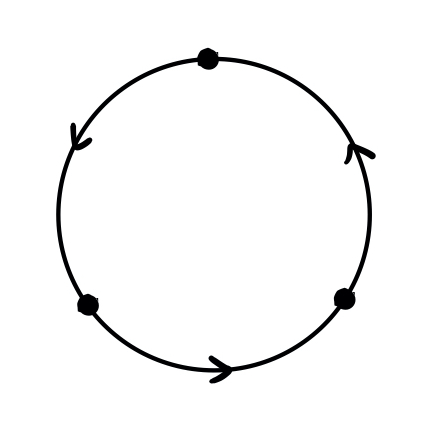
\includegraphics[
      width = 3cm
    ]{delta_complexes1.jpeg}
  \end{figure}
  The sets are : 
  \begin{itemize}
    \item $X_0 := \set{v_0, v_1, v_2}$, representing the three maps 
    of $0$-simplex into this space at the three vertices.
    \item $X_1 := \set{e_0, e_1, e_2}$, representing the three maps 
    of $1$-simplex into this space at the three edges.
    \item $X_n := \nothing$ for $n \geq 2$, representing the fact that 
    there are no (injective) maps of $n$-simplex into this space.
  \end{itemize}
  Now, how these simplices are put together. 
  \begin{itemize}
    \item For $n = 0$. 
    \begin{itemize}
      \item $X(\uparrow_0^0) : X_1 \to X_0, e_0, e_1, e_2 \mapsto 
      v_1, v_2, v_0$. 
      This represents the fact that when viewed as maps 
      from the $1$-simplex into $X$,
      $e_0,e_1,e_2$ restrict to $v_1,v_2,v_0$ along $\uparrow_0^0$.
      \item $X(\uparrow_0^1) : X_1 \to X_0, e_0, e_1, e_2 \mapsto 
      v_0, v_1, v_2$.
      This represents restriction along $\uparrow_0^1 : [0] \to [1]$,
      i.e. picking out the starting point.  
    \end{itemize}
    \item For $n \geq 1$, there's nothing to do. 
  \end{itemize}
  This defines $X = (X_n) \in \De\SET$. 
  Note that in $X$,
  every $n$-face is determined uniquely by 
  its set of vertices.
  These are called \emph{simplicial complexes}.
  Historically, this was one of the candidate definitions
  for ``space made of triangles'',
  however this is ``too rigid'' in the sense that 
  it may take \emph{a lot} of simplices to ``approximate a space",
  so it is impractical for computations.
  An ``approximation using a simplicial complex'' is called a 
  \emph{triangulation}.
  
\end{eg}

\begin{eg}[Boundary of circle, in one piece]
  The picture is 
  \begin{figure}[H]
    \centering
    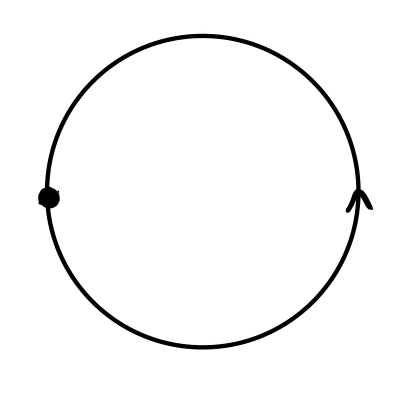
\includegraphics[
      width = 3cm
    ]{delta_complexes2.jpeg}
  \end{figure}
  This demonstrate why delta sets are better than simplicial complexes
  in terms of computation. 
\end{eg}

\begin{eg}[$n$-simplices themselves]
  The picture is of the $2$-simplex, which we'll denote with $\De_2$.
  \begin{figure}[H]
    \centering
    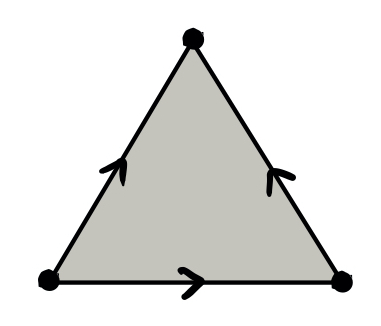
\includegraphics[
      width = 3cm
    ]{delta_complexes3.jpeg}
  \end{figure}
  For $n \geq 3$, we have no ways of mapping the $n$-simplex 
  (injectively) into $\De_2$.
  For $n = 2$, we have one way, which corresponds to the identity. 
  So define $(\De_2)_2 := \set{\id{[2]}}$.
  Restricting this to the boundary edges by omitting vertices 
  gives the three ways of mapping the $1$-simplex
  into $\De_2$.
  This amounts to defining $(\De_2)_1 := 
  \set{\uparrow_1^0, \uparrow_1^1, \uparrow_1^2}$ and 
  for \begin{align*}
    X(\uparrow_1^0) : \id{[2]} \mapsto \uparrow_1^0 \\
    X(\uparrow_1^1) : \id{[2]} \mapsto \uparrow_1^1 \\
    X(\uparrow_1^2) : \id{[2]} \mapsto \uparrow_1^2
  \end{align*}
  These then restrict in two ways to give 
  the three ways of mapping the $0$-simplex into $\De_2$.
  In other words, we define $(\De_2)_0 := \set{(0),(1),(2)}$
  where the elements represent mapping $0$-simplex into 
  the $0$-th, $1$-st, and $2$-nd vertex.
  It follows naturally to define : 
  \begin{align*}
    X(\uparrow_0^0) : \uparrow_1^0, \uparrow_1^1, \uparrow_1^2
    \mapsto (2), (2), (1) \\
    X(\uparrow_0^1) : \uparrow_1^0, \uparrow_1^1, \uparrow_1^2
    \mapsto (1), (0), (0)
  \end{align*}
  This finishes the definition of $\De_2 \in \De\SET$.
  The curious thing is the following, which you may or may not have noticed :
  \emph{$\De_2$ is exactly $\De(-,[2])$, the functor of 
  morphisms into $[2]$}.

  It's not hard to see that more generally,
  the delta set representing the $n$-simplex is 
  $\De(-,[n])$, which we will denote with $\De_n$.
  This gives a functor 
  $\De \to \De\SET, [n] \mapsto \De_n$,
  which is an example of the \emph{Yoneda embedding}.\footnote{
    Embedding means full and faithful.
  }
  The point it makes is the following : 
  We began making spaces out of simplices by axiomatizing simplices.
  But simplices themselves ought to be spaces made of simplices.
  In particular, the $n$-simplex is made exactly by 
  putting together simplices according to how they map into the $n$-simplex.

  A conceptual exercise is to prove \emph{Yoneda's lemma} for 
  $\De$-sets : 
  Let $X \in \De\SET$ and $[n] \in \De$.
  Then we have a bijection of sets, functorial in both $X$ and $[n]$,
  \[
    \De\SET(\De_n, X) \iso X_n
  \]
  The right is what we thought of as the morphisms 
  from the $n$-simplex into $X$,
  and the left is \emph{actual} morphisms from the $n$-simplex into $X$,
  that is, as $\De$-sets.
\end{eg}

\begin{eg}[A portion of an $n$-simplex] 
  The following is a picture of a portion of $\De_2$.
  \begin{figure}[H]
    \centering
    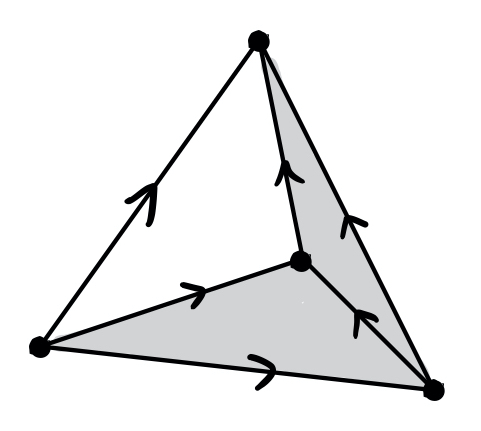
\includegraphics[
      width = 3cm
    ]{delta_complexes4.jpeg}
  \end{figure}
  Writing this up as a $\De$-set $X$,
  one should see that it is a $\De$-subset of $\De_2$.
  In topos theory, subfunctors of Yoneda embeddings of objects
  are also called \emph{sieves}.
  This example demonstrates how you can think of sieves as 
  ``picking out a portion of the object''.
\end{eg}

\begin{eg}[A slightly more elaborate shape]
  (Stolen from alg top cw3.)
  \begin{figure}[H]
    \centering
    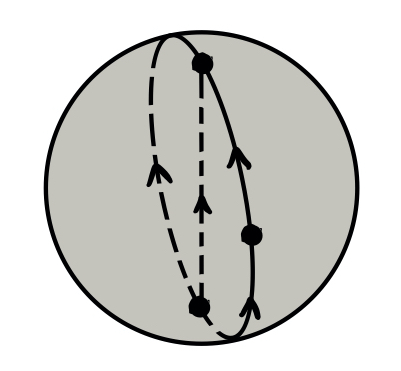
\includegraphics[
      width = 3cm
    ]{delta_complexes5.jpeg}
  \end{figure}
  This is meant to have two faces,
  four edges, and two vertices.
  One of the edges is meant to be ``a pole inside the sphere''.
\end{eg}
\begin{eg}[A non-example]
    Ice cream cone.
    One face, two edges, and two vertices.
    \begin{figure}[H]
      \centering
      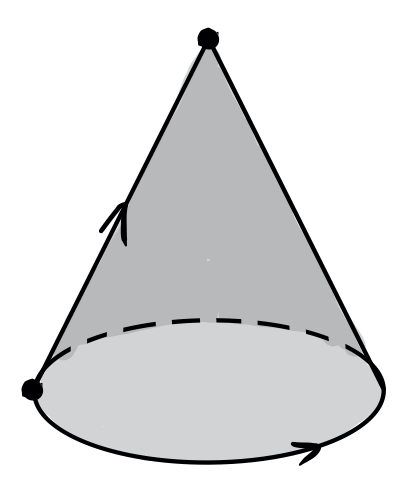
\includegraphics[
        width = 3cm
      ]{delta_complexes6.jpeg}
    \end{figure}
    The reason that this \emph{cannot} be written as a $\De$-set is that 
    one of the restrictions of the unique face is a 
    \emph{``degenerate'' edge}.
    It has been collapsed to the point in the bottom left,
    which we will call $v_0$.
    What happens if one forcefully adds a third edge $\bar{e}$ 
    from $v_0$ to itself, trying to represent the ``degenerate'' edge?
    All this does is add a loop around $v_0$, 
    changing the shape.
    \begin{figure}[H]
      \centering
      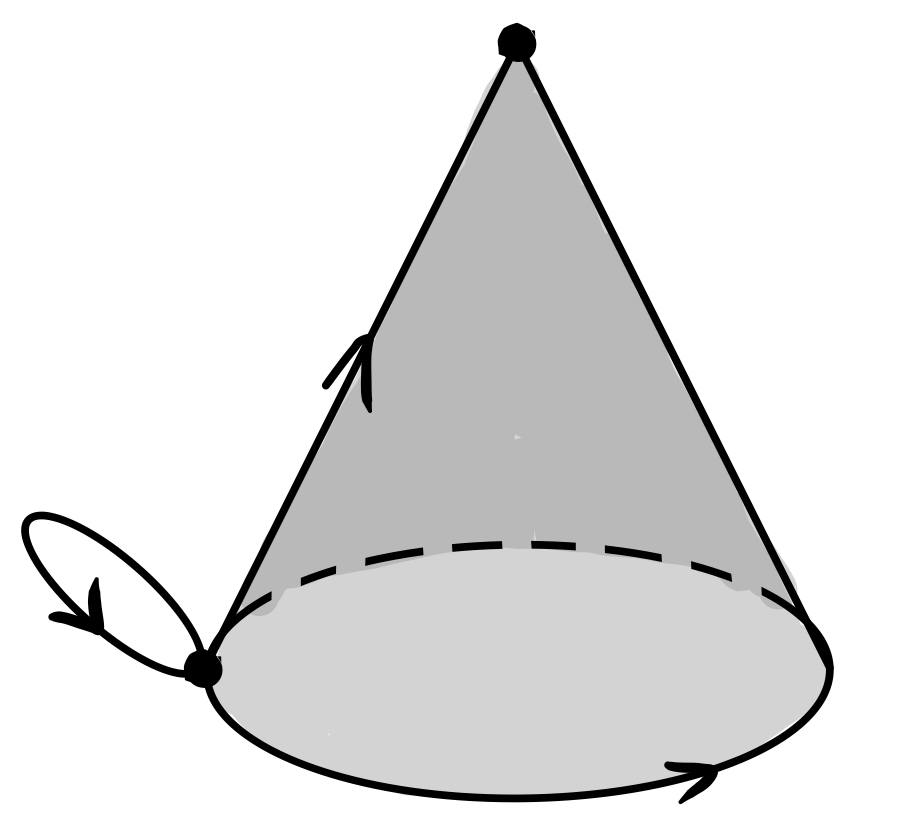
\includegraphics[width = 3.5cm]{delta_complexes7.jpeg}
    \end{figure}
    We could try and ``fill in'' this loop by 
    adding in a face, but then we just need to add 
    more ``degenerate'' edges for the boundaries of the filled in loop, 
    which requires more faces, and so on.

    The point of this example is to show that 
    $\De$-sets don't have enough data to describe ``degenerate'' $n$-faces.
    By throwing in all the ``degenerate'' $n$-faces that ``should be there'',
    one obtains exactly a \emph{simplicial set}.
    This is nice, 
    but as this example hopefully have demonstrated,
    \emph{there will suddenly be a lot of faces},
    which again makes computation unwwieldy. 
    For this reason, we do not pursue simplicial sets further in this 
    document.\footnote{
      I will however remark that 
      it should be true that the data of a simplicial set is
      \emph{essentially} given by all its ``non-degenerate'' faces. 
      This should appear in the form of a 
      fully faithful functor from $\De\SET$ to $s\SET$,
      the category of simplicial sets.
    } 
\end{eg}

\begin{rmk}[Realising $\De$-Sets]
  We discussed before how to realize 
  the simplices by $\abs{\,\cdot\,} : \De \to \TOP, [n] \mapsto \abs{\De_n}$.
  We now show how this extends to $\abs{\,\cdot\,} : \De\SET \to \TOP$
  and the fundamental result that links 
  the two philosophies of ``making spaces out of simplices''.
\end{rmk}

\begin{prop}[Adjunction of Geometric Realisation and Nerve]
  
  For $X \in \TOP$, 
  we define \emph{$\De$-approximations\footnote{
    This is non-standard terminology.
    } of $X$} as 
  $\De$-subsets of the $\De$-set $\TOP(\abs{\,\cdot\,}, X)$
  of all topological morphisms 
  of the realisations of simplices into $X$.
  In algebraic topology,
  the largest $\De$-approximation, $\TOP(\abs{\,\cdot\,}, X)$ itself,
  is called the \emph{singular $\De$-set of $X$},
  often denoted with $S(X)$.
  In category theory, 
  it is called the \emph{nerve of $X$},
  often denoted with $N(X)$.
  We follow the latter notation.
  This defines a functor $N : \TOP \to \De\SET$ called the 
  \emph{nerve functor}.

  Define the functor $\abs{\,\cdot\,} : \De\SET \to \TOP$ as follows : 
  \begin{itemize}
    \item (On objects) Let $X \in \De\SET$.
    We build $\abs{X}$ inductively : 
    define the \emph{zero skeleton of $X$} as 
    $\abs{X}_0 := X_0$ the discrete space.
    Then define the \emph{$(k+1)$-skeleton of $X$} 
    by the pushout diagram in $\TOP$ : 
    \begin{cd}
      \abs{X}_k \ar[r]
        & \abs{X}_{k+1} \\
      \sum_{\si \in X_{k+1}} \sum_{l = 0}^{k+1} \abs{\De_k}
      \ar[r] \ar[u]
        & \sum_{\si \in X_{k+1}} \abs{\De_{k+1}} \ar[u]
    \end{cd}
    where the left vertical arrow is from the UP of coproduct and 
    the construction of $\abs{X}_k$,
    and the bottom horizontal arrow is from the UP of the coproduct and 
    the mappings $\abs{\uparrow_k^0},\dots,\abs{\uparrow_k^{k+1}} : 
    \abs{\De_k} \to \abs{\De_{k+1}}$.

    Finally, the \emph{geometric realisation of $X$} is defined as 
    the colimit $\abs{X} := \COLIM_{k \in \N} \abs{X}_k$.
  \item (On morphisms) induced by UPs.
  \end{itemize}
  The functor $\abs{\,\cdot\,} : \De\SET \to \TOP$ is called 
  \emph{geometric realisation}.

  Then we have the following : 
  \begin{enumerate}
    \item Geometric realisation extends the standard realisation of 
    simplices, meaning we have the following commuting triangle of functors : 
    \begin{cd}
      \De \ar[d,"\De(-)"{swap}] \ar[r,"\abs{\,\cdot\,}"]
        & \TOP \\
      \De\SET \ar[ru,"\abs{\,\cdot\,}"{swap}]
        & 
    \end{cd}
    \item (Adjunction) For $X \in \De\SET$ and $Y \in \TOP$,
    we have the following bijection, functorial in $X$ and $Y$ : 
    \[
      \TOP(\abs{X},Y) \iso \De\SET(X,\TOP(\abs{\,\cdot\,},Y))
    \]
    i.e. a topological morphism from the geometric realisation 
    of $X$ to $Y$ consists of the same data as 
    a choice of topological morphism 
    $\abs{\De_n} \to Y$ for each $n$-face in $X$ 
    ``according to the blueprint of how to make $X$ out of simplices''. 
  \end{enumerate}
\end{prop}
\begin{proof}
  \textit{(1)} Easily checked.
  \textit{(2)} There's a category-theoretic proof using 
  the so-called \emph{density theorem}, which is a small step away from 
  Yoneda's lemma. 
  However, giving the explicit bijection is equally easy, enlightening,
  and ultimately, tautological.
  
  We describe the forward map.
  Let $\ph \in \TOP(\abs{X},Y)$ and let 
  $\ph^\sharp \in \De\SET(X,\TOP(\abs{\,\cdot\,},Y))$ be the corresponding 
  morphism of $\De$-sets we are about to define.
  The map of sets $(\ph^\sharp)_n : X_n \to \TOP(\abs{\De_n},Y)$ is 
  defined by mapping $\si \in X_n$ to the composition : 
  \[
    \abs{\De_n} \to \sum_{\si \in X_n} \abs{\De_n}
    \to \abs{X_n} \to \abs{X} \overset{\ph}{\to} Y
  \]
  This is easily checked to define a morphism of $\De$-sets.
  
  We also describe the inverse map. 
  Let $\al \in \De\SET(X,\TOP(\abs{\,\cdot\,},Y))$.
  To define a map $\abs{X} \to Y$,
  it suffices to give a compatible system of topological morphisms 
  $\abs{X}_n \to Y$.
  Define this inductively. 
  For $n = 0$, $\abs{X}_0 \to Y$ is defined as $\al_0$.
  For $n = k+1$, define $\abs{X}_{k+1} \to Y$ by using its UP as pushout.

  Checking these are inverses and are functorial in $X, Y$ is straightforward.
  It is a good exercise to be able to ``see'' that these are inverses
  and functorial in $X,Y$ without writing out all the details.

\end{proof}

\begin{rmk}
  The motivation of the next definition is evident.
\end{rmk}

\begin{dfn}[Good $\De$-Approximations]
  
  Let $X \in \TOP$.
  A \emph{good $\De$-approximation\footnote{
    Non-standard terminology.
  } for $X$} is a $\De$-approximation $\tilde{X}$ of $X$ such that 
  the corresponding topological morphism $\tilde{\abs{X}} \to X$
  under the realisation, nerve adjunction is an isomorphism.
\end{dfn}

\begin{rmk}[``Delta Complexes'']
  In Hatcher, good $\De$-approximations are called 
  \emph{$\De$-complex structures for $X$}.
  The following lemma proves the equivalence with Hatcher's definition.
\end{rmk}

\begin{lem}[Hatcher's Delta Complexes]
  
  Let $X \in \TOP$, $\tilde{X}$ a $\De$-approximation of $X$.
  Then TFAE :
  \begin{enumerate}
    \item $\tilde{X}$ is a good $\De$-approximation for $X$.
    \item We have the two conditions : 
    \begin{itemize}
      \item (Topology) For all subsets $U$ of $X$,
      $U$ is open if and only if for all $[n] \in \De$ and 
      $\si \in \tilde{X}_n$, $\si\inv U \subs \abs{\De_n}$ is open.
      \item (Bijective) For all $[n] \in \De$ and $\si \in \tilde{X}_n$, 
      $\si : \overset{\circ}{\abs{\De_n}} \to X$ is injective. 
      Furthermore, 
      for all $x \in X$, 
      there exists a unique $[n] \in \De$ and $\si \in \tilde{X}_n$ such that 
      $x \in \si \overset{\circ}{\abs{\De_n}}$.
    \end{itemize}
  \end{enumerate}
\end{lem}
\begin{proof}
  The proof essentially comes down to studying the structure of 
  $\tilde{\abs{X}}$.

  $(1 \implies 2)$ WLOG $X = \tilde{\abs{X}}$.
  We first note that in the definition of $\tilde{\abs{X}}_{k+1}$ : 
  \begin{cd}
    \tilde{\abs{X}}_k \ar[r]
      & \tilde{\abs{X}}_{k+1} \\
    \sum_{\si \in \tilde{X}_{k+1}} \sum_{l = 0}^{k+1} \abs{\De_k}
    \ar[r] \ar[u]
      & \sum_{\si \in \tilde{X}_{k+1}} \abs{\De_{k+1}} \ar[u]
  \end{cd}
  since the bottom horizontal arrow is an isomorphism 
  onto a subspace, 
  so is the top horizontal arrow.
  Then since each $\tilde{\abs{X}}_k \to \tilde{\abs{X}}_{k+1}$ is 
  an isomorphism onto a subspace and 
  $\tilde{\abs{X}}_0 \to \tilde{\abs{X}}_1 \to \cdots$
  is a filtered system,
  it follows that each morphism 
  $\tilde{\abs{X}}_k \to \tilde{\abs{X}}$ is an isomorphism 
  onto a subspace.

  \textit{(Topology)}
  By our construction of $\abs{\tilde{{X}}}$,
  $U \subs X$ is open if and only if for all $[n] \in \De$,
  the preimage of $U$ in $\tilde{\abs{X}}_n$ is open. 
  Then by the inductive construction of $\tilde{\abs{X}}_{k+1}$ as a pushout,
  it can be proven using induction that the above is equivalent to 
  $\si\inv U \subs \abs{\De_n}$ being open for all $\si \in \tilde{{X}}_n$
  for all $[n]$.
  
  \textit{(Bijective)} 
  Let $x \in \tilde{X}$.
  Viewing each skeleta $\tilde{\abs{X}}_k$ as a subspace of $\tilde{\abs{X}}$,
  we have $\tilde{\abs{X}} = \bigcup_{k} \tilde{\abs{X}}_k$.
  For any $k \in \N$,
  we note that the composition 
  \[
    \sum_{\si \in \tilde{X}_{k+1}} \overset{\circ}{\abs{\De_{k+1}}} \to
    \sum_{\si \in \tilde{X}_{k+1}} \abs{\De_{k+1}} \to \tilde{\abs{X}}_{k+1}
  \]
  is again an isomorphism onto a subspace and hence we have \[
    \tilde{\abs{X}}_{k+1} = \tilde{\abs{X}}_k + 
    \sum_{\si \in \tilde{X}_{k+1}} \overset{\circ}{\abs{\De_{k+1}}}
  \]
  where we viewed 
  $\sum_{\si \in \tilde{X}_{k+1}} \overset{\circ}{\abs{\De_{k+1}}}$
  as a subspace of $\tilde{\abs{X}}_{k+1}$.
  It follows that $\tilde{\abs{X}} = \sum_{[k] \in \De} 
  \sum_{\si \in X_{k}} \overset{\circ}{\abs{\De_k}}$,
  from which the desired result is easily seen. 
  
  $(2 \implies 1)$
  As seen above, \textit{(Bijective)} implies 
  the topological morphism $\tilde{\abs{X}} \to X$ is bijective.
  Then \textit{(Topology)} ensures the morphism is a topological isomorphism.

\end{proof}

%\printbibliography

\end{document}